%!TEX root = main-ugly.tex
We slightly adapt the notation used in \cite{khammash1990stability}.  We use Latin letters to denote vectors and matrices, e.g., $Ax = b$, and bold-face Latin letters to denote signals and operators, e.g., $\tf x = (x_t)_{t=0}^\infty$, and $\tf y = \tf G \tf u$.  We let $\ell_\infty$ denote the space of all bounded sequences of real numbers, i.e., $\tf x = (x_t)_{t=0}^\infty \in \ell_\infty$ if and only if $\sup_t |x_t|<\infty$, in which case we define $\linfnorm{\tf x} = \sup_t |x_t|$.  Similarly, we let $\ell^q_\infty$ denote the space of all $q$-tuples of elements of $\ell_\infty$: if $\tf x = (\tf x^1, \dots, \tf x^q) \in \ell^q_\infty$, then $\linfnorm{\tf x} = \max_{i=1,\dots, q}\linfnorm{\tf x^i}$.  We also define the extended space $\ell^{q}_{\infty,e}$ which is equal to the space of all $q$-tuples of sequences of real numbers.  We let $\tf S_+$ denote the right shift operator such tht if $\tf x = (x_t)_{t=0}^\infty$, then $\tf S_+\tf x = (0,x_0, x_1, \dots)$.  Similarly, we let $\tf S_-$ denote the left shift operator such that $\tf S_- \tf x = (x_1,x_2, \dots)$.  Hence $S_-S_+ = I$, but in general $S_+ S_- \neq I$.  

We let $\LTV^{p,q}$ be the space of all bounded linear causal operators mapping $\ell^q_\infty \to \ell^p_\infty$, and broadly refer to all such operators as $\ell_\infty$-stable.  If $\tf R \in \LTV^{p,q}$, then $\linffnorm{\tf R} := \sup_{\linfnorm{\x}\leq 1}\linfnorm{\tf R \tf x}$, which is the induced operator norm.  Note that each $\tf R \in \LTV^{p,q}$ can be completely characterized by its block lower-triangular pulse response matrix.  We denote by $\LTI^{p,q}$ the subspace of $\LTV^{p,q}$ consisting of time-invariant operators, and further denote by $\RHinf^{p,q}$ the subspace of $\LTI^{p,q}$ consisting of all stable finite-dimensional systems.  When the dimensions can be inferred from context, they will be omitted.  We use $z$ to denote the discrete-time z-transform variable: it follows that the restriction of $\Sp$ to $\LTI$ is given by $\frac{1}{z}$, and similarly the restriction of $\Sm$ to $\LTI$ is given by $z$.  Finally, we recall that an operator $\tf G \in \LTI^{p,q}$ is uniquely characterized by its $z$-transform $\tf G(z) = \sum_{i=0}^\infty z^{-i}G_i$ -- when there is no confusion, we will use $\tf G$ to denote both the operator and its $z$-transform.

\begin{figure}
\centering
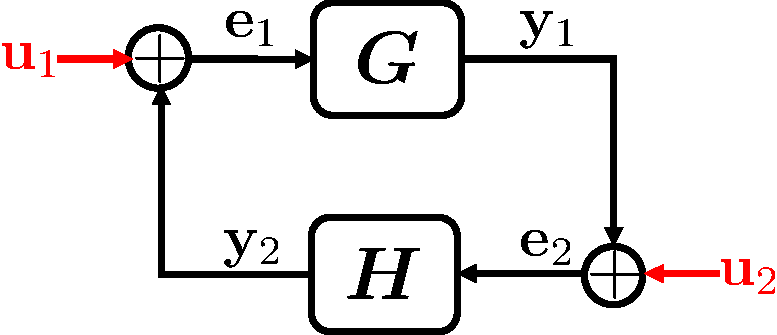
\includegraphics[width=.4\columnwidth]{well-posed}
\caption{A feedback interconnection between systems $\mathbf{G}$ and $\mathbf{H}$.}
\label{fig:well-posed}
\end{figure}


The feedback interconnection as in Fig. \ref{fig:well-posed}, where $\mathcal{G}: \ell_{\infty,e}^p \to \ell_{\infty,e}^q$ and $\mathcal{H}: \ell_{\infty,e}^q \to \ell_{\infty,e}^p$, is \emph{well-posed} if $(I-\mathbf{GH})^{-1}$ exists as a map from $\ell_{\infty,e}^q \to \ell_{\infty,e}^q$, and it is $\ell_\infty$-stable if it is (i) well posed, (ii) the map $(\uu_1,\uu_2) \to (\tf{e}_1,\tf e_2, \tf y_1, \tf y_2)$ takes $ \ell_{\infty}^p \times \ell_{\infty}^q$ into $\ell_{\infty}^p \times \ell_{\infty}^q \times \ell_{\infty}^p \times \ell_{\infty}^q$, and (iii) there exist constants $\alpha_1$ and $\alpha_2$, independent of $\uu_1$ and $\uu_2$, such that $\max\left\{\linfnorm{\tf e_1},\linfnorm{\tf e_2},\linfnorm{\tf y_1},\linfnorm{\tf y_1}\right\} \leq \alpha_1\linfnorm{\uu_1}+\alpha_2\linfnorm{\uu_2}$.  Similarly, a map $\tf G:\ell_{\infty,e}^q \to \ell_{\infty,e}^p$ is $\ell_\infty$-stable if it is causal, takes $\ell_\infty^q$ into $\ell_\infty^p$, and is bounded, i.e., $\linffnorm{\tf G} < \infty$ or equivalently, $\tf G \in \LTV^{p,q}$.  Necessary and sufficient conditions for the interconnection in Fig. 1 to be $\ell_\infty$-stable are then that $\tf G$ and $\tf H$ are $\ell_\infty$-stable, that the interconnection is well-posed, and that $(I-\tf G \tf H)^{-1}$ is $\ell_\infty$-stable.  We note that it is sufficient to verify that only $(I-\tf G \tf H)^{-1}$ is $\ell_\infty$-stable as it is easily shown that this is true if and only if $(I-\tf H \tf G)^{-1}$ is $\ell_\infty$-stable (see Proposition 1, \cite{khammash1990stability}).  Finally we note that in the case of finite dimensional linear-time-invariant (LTI) systems, the interconnection in Fig. \ref{fig:well-posed} is $\ell_\infty$-stable if and only if it is \emph{internally stable}.